\documentclass[a4paper,10pt]{article}
\usepackage[utf8x]{inputenc}
\usepackage{graphicx}
\usepackage{minted}

%opening
\title{\textit{Java Behaviour Trees}, a Java Framework for Creating and Running Behaviour Trees}
\author{Ricardo Juan Palma Dur\'an}

\begin{document}

\maketitle

\begin{abstract}

Behaviour Trees (BTs) have gained popularity over the past few years as a tool for defining the behaviour of video games' characters. However, to the best of our knowledge, currently there is no open Java implementation of BTs. Here we present \textit{Java Behaviour Trees} (JBT), a GNU framework in Java for defining and running BTs.

\end{abstract}

\section{Introduction}

We assume that the reader is familiar with the concept of BT. Here we are not going to explain all the details about what a BT is or how it conceptually works. Some authors have spent a lot of effort doing so, so we will just refer the reader to \cite{Millington09} for an introduction.

The model we have implemented is a hybrid one, since it combines ideas from several sources. The basic underlying model is that of \cite{Millington09}, including all the task that the authors propose as well as the concept of context and libraries of behaviour trees. However, we have also added \textit{guards} to our implementation. Guards act like conditions that in some scenarios are checked in order to decide whether a task is run or not. 

We have also taken some ideas from \cite{AIGameDev}, specially that of having trees whose nodes are ticked only when necessary so that CPU time does not get wasted.

\subsection{Model overview description}

In this section we describe the JBT architecture as well as the main features that BTs have.

\subsubsection{Model driven by ticks}

JBT implements a BT model driven by ticks. A BT must be evaluated through ticks, so every game cycle an external caller \textit{ticks} the tree in order for the tree to update its status. A tick is just a way of giving the tree some CPU time to update their status; in particular, ticks are used to give the nodes of the tree some time to evaluate whether they have finished or not, and consequently make the tree evolve.

The simplest approach to BTs driven by ticks is that of ticking the root node and then letting each node recursively tick its children according to its semantics. However, this is a very inefficient process, since in general the major part of the nodes of the tree are just waiting for their children to finish. Therefore, they should not receive ticks, since unless their children are done they will do nothing useful when receiving the tick. Therefore, in general only very few nodes should be ticked at a game cycle, and as a result JBT implements a model in which there is a list of \textit{tickable} nodes. Only the nodes in the list can be ticked.

\subsubsection{Model independent from execution}

When running a BT, there should be a clear distinction between the tree that is being run (the model) and how it is actually being run (the execution). For each particular behaviour, we distinguish between the \textit{Model BT} that defines it and how it is being run. The \textit{how} is what the \textit{BT Executor} does. Basically, for every entity in the game that wants to run a behaviour (Model BT), there is a BT Executor. The BT Executor takes the Model BT and processes it (without modifying it), simulating the behaviour that is represented by the Model BT. This choice implies that, apart from the Model BT, there is another type of tree, the \textit{Execution BT}. When an entity wants to execute a behaviour, the BT Executor takes the Model BT and creates an Execution BT to execute the behaviour. The BT Executor along with the Execution BT know how to run the behaviour that the Model BT represents.

\subsubsection{Architecture}

Figure \ref{fig:Overview} shows an overview of the proposed architecture for BTs. There is a Model BT that represents a particular behaviour. Also, there is a BT Executor for every entity that wants to run the Model BT. Each BT Executor makes use of the Model BT and builds an Execution BT that actually runs the behaviour conceptualized by the Model BT. An external Game AI ticks the BT Executors, in order for them to update the trees that they are running.

\begin{figure}
 \centering
 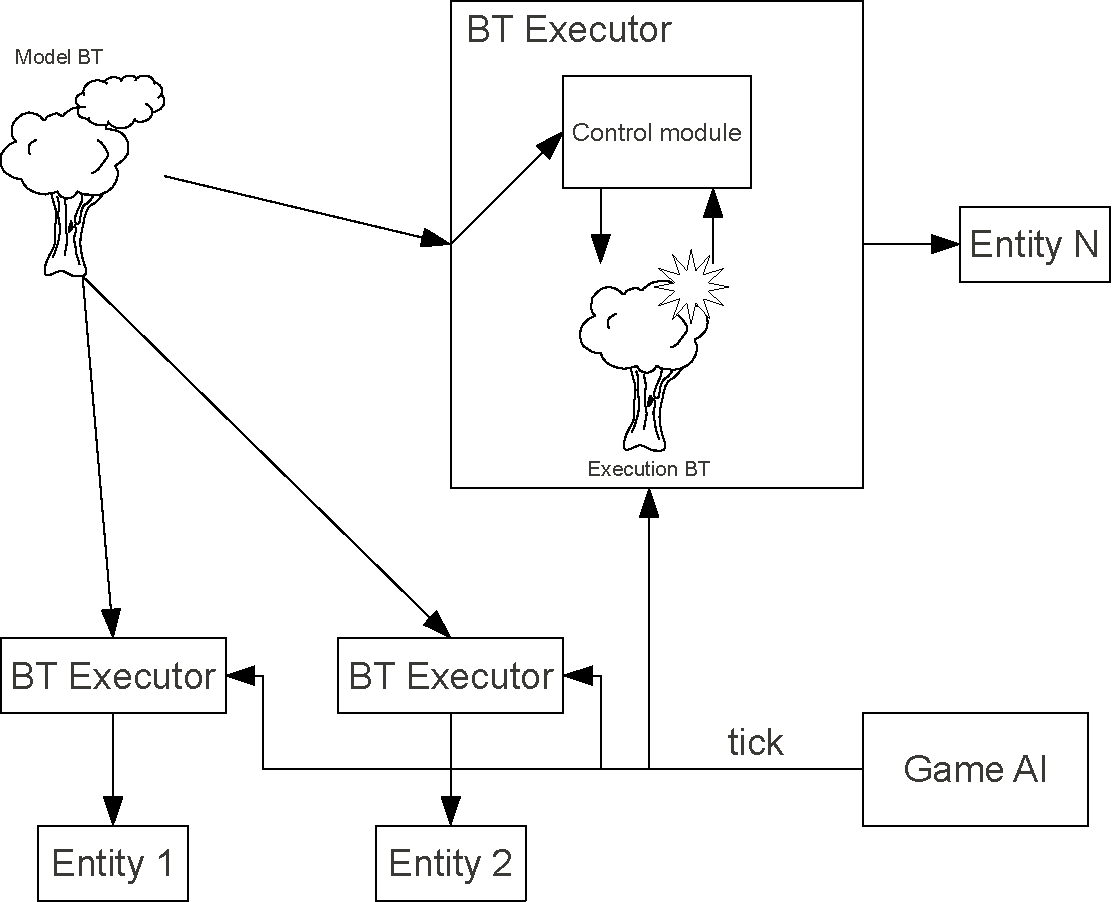
\includegraphics[width=\textwidth]{./Images/Overview.pdf}
 \caption{Overview of the BT architecture}
 \label{fig:Overview}
\end{figure}

\section{Lists of nodes}

At all times, the BT Executor receives ticks from an external Game AI. As a consequence, the BT Executor makes the tree it contains evolve.

Not all the nodes of the tree should receive ticks. In general, the evolution of the tree depends on a very small set of nodes, which, in general, is mainly composed of leaves of the tree. In general, intermediate nodes, such as sequences or selectors, should do nothing unless they are notified by their children after finishing. As a consequence, it is obvious that only a few nodes should receive ticks. The rest should be somehow \textit{asleep}, waiting for some events to take place in order to be awakened.

We have implemented an architecture where, for each BT being run, there is a list of \textit{tickable nodes} (\textit{Tickable Nodes List} from now on). Whenever the external Game AI ticks the BT Executor, the BT Executor will only tick the nodes in the Tickable Nodes List. This list is modified through out the execution of the tree, so nodes enter and leave the list depending on whether they are useful with respect to the evolution of the tree or not.

Also, at all times the BT Executor knows which nodes are open (or active). A node is active if it belongs to a path from the root node to an active leaf node. Therefore, open nodes represent those that are actively involved in the current execution of the tree. They may not be tickable nodes, but the fact that they belong to a path from the root to an active leaf node means that they may receive ticks soon.

This list is called the \textit{Open Nodes List}.

\section{Model BT, guards and context}

A Model BT is a BT that conceptually represents a behaviour. A Model BT does not have running capabilities, that is, it is just a way of defining a behaviour. An external interpreter, the BT Executor, uses the Model BT as a base to run the behaviour it embodies. A Model BT is shared by all the entities that want to run such a behaviour. By following this model, there is only one tree even though it is being actually run by several entities.

The main functionality of a Model BT is very simple. The base class for a node (also called \textit{task}) is mainly as follows:

\begin{minted}{java}
public abstract class ModelTask{
  /* The list of children of the task. */
  private List<ModelTask> children;

  /* The guard of the task, which may be null. */
  private ModelTask guard;

  public ModelTask(ModelTask guard, ModelTask... children){
    this.children = new Vector<ModelTask>();
    for(int i=0;i<children.lenght;i++){
      this.children.add(children[i]);
    }
    this.guard = guard;
  }

  public List<ModelTask> getChildren(){
    return this.children;
  }

  public ModelTask getGuard(){
    return this.guard;
  }

  ...
}
\end{minted}

That is, a task is just a container of other tasks, with no running capabilities. A task's children can be accessed, as well as its guard. In this model, a behaviour tree is equivalent to a ModelTask object, that is, a ModelTask can be interpreted as the behaviour tree whose root is the ModelTask itself. There can be as many ModelTask subclasses as supported by the underlying BT model being implemented, but none of them should define running methods.

A guard is represented by an ModelTask object. Initially, we defined guards as objects implementing the \textit{IGuard} interface:

\begin{minted}{java}
public interface IGuard{
  /* Evaluates the guard within a context. */
  public boolean evaluate(IContext);
}
\end{minted}

That is, a guard was just an entity capable of being evaluated within a context, issuing a boolean value as a result. However, a more general approach is that of considering a ModelTask to be a guard. By doing so, \textit{conditions} (ModelTasks that evaluate certain attributes of the world) can be used as guards. What is more, any behaviour tree can be used as a guard. As long as the behaviour tree succeeds, the guard evaluation is interpreted as \textit{true}; if the behaviour tree fails, the guard evaluation is interpreted as \textit{false}.

In general, guards will be implemented by single ModelTask nodes. For instance, if a guard has to check if the current player has enough resources to build a particular type of unit, then a subclass of ModelTask may represent such condition. This conditions may be used, not only as a guard, but also as a condition node along the tree.

The main advantage of this method is that of reusability, since predefined tasks can also be used as guards.

A context is defined by the \textit{IContext} interface:

\begin{minted}{java}
public interface IContext{
  /* Sets the value of a variable. */
  public void setVariable(String name, Object value);

  /* Gets the value of a variable (null if not found). */
  public Object getVariable(String name);

  ...
}
\end{minted}

We will extend this interface further in following sections. However, the previous two methods define the core of what a context should be in a behaviour tree: an large repository of variables that can be modified an accessed by tasks.

\section{Execution BT and BT Executor}\label{Sub:ExecutionBTAndBTExecutor}

An Execution BT is a BT capable of running a particular BT Model. The idea behind this whole architecture is that, for each ModelTask, there must be another task knowing how to run it. For instance, there could be an ExecutionSequenceTask knowing how a ModelSequenceTask behaves, or an ExecutionParallelTask knowing how to run a ModelParallelTask. 

\textit{ExecutionTask} is the base class for all the tasks with the ability to run. An ExecutionTask has a reference to the ModelTask it represents, so it knows what the structure of the conceptual tree is like. An ExecutionTask also has a reference to the BT Executor in charge of it.

The BT Executor contains the Tickable Nodes List and the Open Nodes List. Both lists store ExecutionTasks.

Initially, the BT Executor receives the Model BT it should execute. It then creates an ExecutionTask for the root node of the tree, and \textit{spawns} it. When an ExecutionTask is spawned, it recursively spawns its children according to the semantics of the particular task. The idea is that, when \textit{spawn()} is called, the path(s) containing all the tasks from the root to the active leaf nodes must be created and stored. When a task is spawned, it has to decide whether it enters the list of tickable nodes or not. Also, when a task is spawned, it is inserted into the \textit{Open Nodes List}.

From then on, the BT Executor just ticks the list of tickables nodes it contains. At every tick, the tickable nodes analyse their current situation to check whether they have or have not finished. For an intermediate node, this decision in general depends on whether its children have finished or not. For leaf nodes, this decision usually depends on an external process that has to be checked for termination.

When a task (intermediate or not) has finished, it should notify its parent. In general, parent (intermediate) nodes will not usually be tickables; therefore, they will not be in the Tickable Nodes List, and as a result, the only way for them to notice that they have to be updated is by being explicitly told so. Thus, when a tickable finishes, a TaskEvent is fired. Parents register as TaskEventListeners of their children (at spawning time), so whenever a child is done, the parent will immediately realize and will be able to act as a consequence. By following this pattern, only very few tasks must stay in the Tickable Nodes List: in general, only leaf nodes will receive ticks. When they are done, they will automatically fire a TaskEvent. Parents, on the other hand, will usually register as TaskEventListeners of their children, so they will receive such events and will be able to have a chance to react to the termination of their children. If the parent finishes as a consequence of the child's termination, then the parent will fire a TaskEvent to notify its parent too, and so on.

The BT Executor has a very simple interface:

\begin{minted}{java}
public class BTExecutor{
  /* The Model BT being run. */
  private ModelTask modelBT;

  /* The list of tickable nodes. */
  private List<ExecutionTask> tickableList;

  /* The list of open nodes. */
  private List<ExecutionTask> openList;

  /* Updates the tree being run. */
  public void tick();

  /* Terminates the execution of the tree. */
  public void terminate();

  /* Returns the status of the tree being run. */
  public Status getStatus();

  ...
} 
\end{minted}

An ExecutionTask mainly contains a reference to the ModelTask it is running, the BTExecutor and the context (IContext), as follows:

\begin{minted}{java}
public abstract ExecutionTask implements ITaskListener{
  /* Reference to the corresponding ModelTask. */
  private ModelTask modelTask;

  /* The BTExecutor that is running this ExecutionTask. */
  private BTExecutor executor;

  /* The context of the task. */
  private IContext context;

  /* List of all the listeners of this task. */
  private List<ITaskListener> listeners;

  /* Current status of the task. */
  private Status currentStatus;

  /* Spawns the task and its children. */
  public final void spawn(IContext context){...};

  /* Ticks the task. */
  public final void tick(){...}
 
  /* Terminates the task. */
  public final void terminate(){...}

  /* Returns the current status of the task. */
  public Status getCurrentStatus(){
    return this.currentStatus;
  }

  /* 
   * Adds a task listener to this task. The
   * task listener will be notified when an important
   * change in the status of this task occurs.
   */
  public void addTaskListener(ITaskListener listener){
    if(listener != null){
      this.listener.add(listener);
    }
  }

  /* Called to fire the TaskEvent on all the listeners. */
  private void fireTaskEvent(Status s){
    for(ITaskListener t:this.listeners){
      t.taskFinished(new TaskEvent(s));
    }  
  }

  ...
}
\end{minted}

An ExecutionTask has three main methods, \textit{spawn()}, \textit{tick()} and \textit{terminate()}. These three methods define the main functionality of an ExecutionTask. They have a base definition that cannot be overriden by subclasses, and their internal implementation relies upon three abstract methods, \textit{internalSpawn()}, \textit{internalTick()} and \textit{internalTerminate()} respectively. Subclasses define their specific behaviour by implementing these abstract methods.

As stated before, the standard behaviour of all ExecutionTask is implemented in the \textit{spawn()}, \textit{tick()} and \textit{terminate()} methods. Their definition is as follows:

\begin{minted}{java}
/* Spawn. */
public final void spawn(IContext context){
  /*
   * Store the context.
   */
  this.context = context;

  /* Set the current status of the task to Status.RUNNING. */
  this.status = Status.RUNNING;

  /*
   * Request to be inserted into the list of open tasks.
   */
  this.executor.requestInsertionIntoOpenList(this);
  
  /*
   * Carry out the actual spawn.
   */
  internalSpawn();
}

/* Tick. */
public final Status tick(){
  Status newStatus = internalTick();

  this.currentStatus = newStatus;

  if(this.currentStatus != RUNNING){
    this.executor.requestRemovalFromTickableList(this);
    this.executor.requestRemovalFromOpenList(this);

    fireTaskEvent(newStatus);
  } 

  return newStatus;
}

\end{minted}

With respect to the \textit{terminate()} method, see section \ref{Sub:TerminatingTasks} for further explanation. As we can see, the main purpose of \textit{spawn()} is to store the context (so that in is accessible later on, when the task actually needs it) and request that the task be inserted into the list of open nodes. Finally, it calls \textit{internalSpawn()}, where the task will carry out the spawning process according to its semantics (for instance, a parallel task would spawn all of its children, while a selector would spawn just one child). This method is in charge of the following:

\begin{itemize}
  \item It decides whether it should enter the Tickable Nodes List or not\footnote{See Section \ref{Sub:ManagingLists} for further explanation.}. For instance, an ExecutionSequenceTask should not enter the list, because the fact that it evolves or not depends on the termination of its children (therefore, only its children should enter the list). However, low level actions or tasks such as DynamicPriorotyList should. It is very important to note that if the spawning process of a task fails, it should enter the Tickable Nodes List in order for it to notify its parent at the next AI cycle. A DynamicPriorityList, for instance, may fail in case no valid guard is found, in which case it should be ticked at the next AI cycle so as to notify its parent.

  \item According to the semantics of the node, it recursively spawns none, one or several of its children. For instance, an ExecutionSequenceTask should spawn the very first node of its list of children. An ExecutionParallelTask should spawn all of its children. On the contrary, a low level task (leaf node) cannot spawn any child since it has none.

  \item In case of a low level task, \textit{internalSpawn()} should start the execution of the process associated to the node. Keep in mind that low level tasks may perform long processes that require several ticks in order to complete. It is in this method that those processes start (maybe in independent threads). It should be noted, however, that many processes may be \textit{instantaneous}, so they may complete even within the \textit{internalSpawn()} method. Nevertheless, in these cases the tree should not evolve, reason why the termination notification to its parent should be carried out in the \textit{tick()} method, in the next AI cycle. If \textit{internalSpawn()} were allowed to notify parents when the node terminated, then a single call to \textit{spawn()} may take too long to complete due to the uninterrupted evolution of the tree, which is something that has to be avoided.
\end{itemize}

On the other hand, \textit{tick()} calls the \textit{internalTick()} method, where the task will carry out the actual ticking process. Then, if the task has finished after calling it, a TaskEvent will be fired to notify all the listeners that are registered with the task, and it requests to be removed from the Tickable Nodes List and the Open Nodes List. It is by this mechanism that parents are notified about their children termination, and can act accordingly.

\textit{internalTick()} is the method that actually performs the tick. In general, this method will analyse the current status of the children of the task (\textit{ExecutionTask.getStatus()}), and will evolve accordingly. For instance, when an ExecutionSequenceTask receives a TaskEvent from its currently active child, its \textit{tick()} method gets called, and the following is done (in \textit{internalTick()}):

\begin{itemize}
\item If the child has succeeded, the ExecutionSequenceTask will spawn the next child in case there is one, and will return RUNNING. In case it is the last child, it will return SUCCESS.
\item If the child has failed, the ExecutionSequenceTask will also fail, returning FAILURE.
\end{itemize}

The ITaskListener interface represents an interface for listening to events fired when there are important changes in the status of a task.

\begin{minted}{java}
public interface ITaskListener{
  /* 
   * Called whenever there is a change in
   * the status of a task. 
   */
  public void statusChanged(TaskEvent e);
}
\end{minted}

In general, the method \textit{statusChanged()} will just call \textit{tick()} on the node itself. By doing so, the node will be able to advance, either by spawning other children or by firing a TaskEvent to its parent to make it go on too.


\section{Creating ExecutionTasks from ModelTasks}

ExecutionTasks must be created for ModelTasks. In order to make this process easier, it can be delegated to ModelTasks. When an ExecutionTask needs to create the ExecutionTask of one of its children, it can ask the corresponding ModelTask to do so. Therefore, ModelTasks define a new method,

\begin{minted}{java}
/* 
 * Creates an ExecutionTask that is able to run 
 * this ModelTask. "executor" is the BTExecutor 
 * managing the ExecutionTask that will be created.
 */
public abstract ExecutionTask createExecutor(BTExecutor executor);
\end{minted}

This method should return an ExecutionTask capable of running the corresponding ModelTask. Keep in mind that the returned ExecutionTask must have a reference to the ModelTask that created it. For instance, in case of a ModelSequenceTask, it should do something like:

\begin{minted}{java}
public ExecutionTask createExecutor(BTExecutor executor){
  return new ExecutionSequenceTask(this, executor);
}
\end{minted}

By following this pattern, it would be ModelTasks that would be in charge of creating ExecutionTasks through \textit{createExecutor()}.


\section{Managing the Tickable Nodes List and the Open Nodes List}\label{Sub:ManagingLists}

When tasks are being ticked, there may be a problem accessing the Tickable Nodes List. The algorithm followed by the BTExecutor is pretty simple:

\begin{minted}{java}
public class BTExecutor{
  ...

  public void tick(){
    if(this.firstTimeCalled){
      ExecutionTask root = this.modelBT.createExecutor();
      root.spawn();
      this.firstTimeCalled = false;
    }
    else{
      for(ExecutionTask t:this.tickableList){
	t.tick();
      }
    }

    ...
  }

  ...
}
\end{minted}

That is, it just ticks all the nodes in the Tickable Nodes List. However, while the list is being ticked, some nodes may need to leave the list, so the iteration through its elements may be left in an inconsistent state. Therefore, when a node wants to enter or leave the list, it does not \textit{immediately} do it. Instead, it \textit{requests} to be inserted or removed. When the BTExecutor has ticked all the nodes, it processes these requests, so the code above should finally be something like:

\begin{minted}{java}
public class BTExecutor{
  ...
 
  public void tick(){
    if(this.firstTimeCalled){
      ExecutionTask root = this.modelBT.createExecutor();
      root.spawn();
      this.firstTimeCalled = false;
    }
    else{
      for(ExecutionTask t:this.tickableList){
	t.tick();
      }
    }
    
    processRemovalsAndInsertions();
  }
  
  ...
}
\end{minted}

In order to prevent the Open Nodes List from failing the same way, insertions and removals from it are also requested and delayed instead of being immediately carried out. 

\section{Terminating tasks}\label{Sub:TerminatingTasks}

In certain cases, tasks must be abruptly terminated. This happens, for instance, when a parallel task realizes that one of its children has failed. In such a case, it has to immediately stop the other children. Another example is when a whole tree needs to be terminated, because it just does not make sense to run it any more. As we can see, there are several scenarios in which it is necessary to have the ability to stop individual tasks or branches of a tree. This is the purpose of the method \textit{terminate()}, first introduced in the section \ref{Sub:ExecutionBTAndBTExecutor}.

As a consequence of these requirements, BTExecutor and ExecutionTask need to be extended, so both include a \textit{terminate()} method. In the case of the BTExecutor, its implementation is trivial: it will just terminate the tree that it is running. However, the \textit{terminate()} method in the ExecutionTask class is more complicated. Since the termination process of an ExecutionTask varies according to the specific type, it is an final method whose implementation relies on the abstract \textit{internalTerminate()} method, which carries out the actual termination process.

What \textit{terminate()} does is to request that the task be removed from both the list of tickable and open nodes, sets the status of the task to \textit{terminated}, and finally calls \textit{internalTerminate()}. For non-leaf tasks, \textit{internalTerminate()} usually calls \textit{terminate()} on their active children, in a recursive manner. For leaf tasks, it will stop and free all the processes and resources belonging to the task.

The problem about terminating tasks is that they must not leave the list of tickable nodes until the next game AI cycle (that is, until \textit{BTExecutor.tick()}) is called again. This is due to the fact that the list of tickable nodes may be being ticked just when a task is terminated. If the terminated task(s) were removed from the list, then it would be left in an inconsistent state and the BTExecutor would have problems ticking all of its tasks. It is for this reason that when a task is requested to terminate itself, the task does not immediately remove itself from the Tickable Nodes List, but requests it. Now, the problem is that the BTExecutor could tick tasks that have been terminated, since they are not removed from the Tickable Nodes List until the current AI cycle finishes.In order to prevent from any problem, the \textit{ExecutionTask.tick()} method is modified so that, if the task has been terminated, it does nothing.

\begin{minted}{java}
public abstract ExecutionTask implements ITaskListener{
  ...
  public Status tick(){
    if(!this.terminated){
      Status newStatus = internalTick();

      this.currentStatus = newStatus;

      if(this.currentStatus != RUNNING){
	requestRemovalFromTickableList(this);
	requestRemovalFromOpenList(this);

	fireTaskEvent(newStatus);
      } 

      return newStatus;
    }
    else{
      return Status.TERMINATED;
    }
  }
  ...
\end{minted}

The \textit{ExecutionTask.terminate()} method is mainly implemented like this:

\begin{minted}{java}
public abstract ExecutionTask implements ITaskListener{
  ...
  public void terminate(){
      if(!this.terminated){
	requestRemovalFromOpenList();
	requestRemovalFromTickableList();
	this.terminated = true;
	this.currentStatus = Status.TERMINATED;
	internalTerminate();
      }
  }
  ...
}
\end{minted}

That is, the \textit{terminate()} method requests to remove the task from both the Open Nodes List and the Tickable Nodes List. Also, it activates a flag to indicate that the task has been terminated. Finally, it calls the abstract method \textit{ExecutionTask.internalTerminate()} which will actually terminate the task.

\textbf{It must be noted that the termination process must be carefully handled}. When a task is terminated, it immediately becomes totally unresponsive, so ticking it will have no effect; also, at the next game AI cycle, it will be removed from the list of tickable nodes. As a result, its parent will never be notified about its child termination -it will not receive a TaskEvent-, and it will never be able to evolve. 

Therefore, when a task is terminated, its parent should enter the list of tickable nodes so that at the next game AI cycle it can receive ticks and realizes that its child has finished (been terminated). This is for example what the ExecutionInterrupter does when it is interrupted: it terminates its child and then requests to be inserted into the list of tickable nodes. Even though it may not be necessary to always insert the parent task into the list of tickable nodes, it should be kept in mind that terminating tasks is a very delicate process that must be properly handled.

\section{General process}

So far we have described a general architecture to model and run behaviour trees. Despite the fact that there are still many details to be taken care of, we can give an overview of the whole process of managing a behaviour tree:

\begin{itemize}

\item A Model BT is created. The Model BT represents the behaviour that must be run, but it cannot be executed by itself. The tree would be implemented by a ModelTask.

\item A BTExecutor is created. The BTExecutor will contain a reference to the ModelTask that must be run.

\item From then on, \textit{BTExecutor.tick()} is called in order to run the tree. At every game cycle, \textit{tick()} is called. The external caller should not worry about anything else; it will be the BTExecutor that will handle the execution of the BT.

\begin{itemize}

\item The very first time \textit{tick()} is called, the BTExecutor takes the root node of the Model BT, and creates the corresponding ExecutionTask node, which is spawned. This is done by calling \textit{ModelTask.createExecutor()}, and then calling \textit{ExecutionTask.spawn()} on the returned ExecutionTask.

\item From then on, every time \textit{BTExecutor.tick()} is called, the BTExecutor will just tick the nodes in the Tickable Nodes List. 

\end{itemize}

\item Whenever a task finishes, it fires an event to inform its parent. The parent will then either report success or failure (depending on whether the child failed or succeeded) or spawn a new child. If the parent also finishes, it will fire a new event to its parent, in a recursive manner.

\end{itemize}

\section{Actions and conditions (leaf nodes)}

Actions and conditions, that is, leaf nodes in the BT, must be somehow specified. At design level, the BT is designed including all the low level actions and conditions that the tree is supposed to run, but in an abstract manner. 

On the implementation side, however, there must be an ExecutionTask that knows how to run each leaf node. Since these tasks are outside the framework, a way of defining their behaviour must be provided. The framework provides two abstract classes, \textit{ModelAction} and \textit{ModelCondition}, so every low level action and condition must subclass them, 

\begin{minted}{java}
public abstract class ModelAction extends ModelTask{
  ...
}
\end{minted}

\begin{minted}{java}
public abstract class ModelCondition extends ModelTask{
  ...
}
\end{minted}

For instance, a low level action \textit{MoveTo} would be defined like this:

\begin{minted}{java}
public class MoveTo extends ModelAction{
  ...
}
\end{minted}

ModelTasks and ModelConditions also define a \textit{createExecutor()} method that must return the corresponding ExecutionTask to run the action or condition. The designer should define the \textit{internalSpawn()}, \textit{internalTick()} and \textit{internalTerminate()} methods for these ExecutionTasks. For instance, lets suppose that the designer has created a BT with a low level action called \textit{MoveTo}. Such action would be represented by two classes:

\begin{minted}{java}
public class ModelMoveTo extends ModelAction{
  ...

  public ExecutionTask createExecutor(BTExecutor executor){
    return new ExecutionMoveTo(this, executor);
  }
}
\end{minted}

\begin{minted}{java}
public class ExecutionMoveTo extends ExecutionAction{
  ...

  public void internalSpawn(){
    /* TODO: designer should implement this method! */
  }

  public Status internalTick(){
    /* TODO: designer should implement this method! */
    return Status.SUCCESS;
  }

  public void internalTerminate(){
    /* TODO: designer should implement this method! */
  }
}
\end{minted}

So the designer should only implement the \textit{internalSpawn()}, \textit{internalTick()} and \textit{internalTerminate()} methods. In the case of the MoveTo action, \textit{internalSpawn()} would send the unit the move order through the game engine. \textit{internalTick()} would check whether the unit has arrived at its destination. If so, it would return \textit{Status.SUCCESS}; otherwise, it would return \textit{Status.RUNNING}.

\section{Evaluation order}

The problem with having a Tickable Nodes List is that the order in which nodes are ticked does not necessarily correspond to that of an ideal BT. Suppose for example that we have a BT with a DynamicPriorotyList (DPL) task, and some of its children are currently running. Suppose an scenario in which, if the active child is ticked, it finishes successfully, but at the same time, if the DPL is ticked, it realizes there is a child with higher priority that must be run.

Ideally, the DPL is ticked first, so it terminates the currently active child and spawns the child with higher priority. However, if in the Tickable Nodes List the currently active child is placed before the DPL node, it will receive a tick first. In the presented scenario, the child would finish with success, the DPL would be informed, and as a result, it would terminate without spawning the child with higher priority. Moreover, the child task would succeeds while in the ideal BT it would not.

This problem can be fixed by forcing an order in the Tickable Nodes List. In particular, if parent nodes always precede their children at ticking time, then this problem is fixed, since by doing so the ideal evaluation order of a BT is emulated.

\section{Subtree Lookup and IContext}\label{sec:SubtreeLookupAndIContext}

One of the most important features of behaviour trees is that of reusability. In the context of behaviour trees it is very important to notice the way that parent tasks interact with their children: parents do not care about what their children are; in JBT, on the conceptual side, this can be seen in the fact that ModelTasks always have other ModelTasks as children, and it is through its interface that they interact, no matter the particular subtype. On the execution side, ExecutionTasks always have other ExecutionTasks as their children, and it is also through its interface that they interact, no matter the particular subtype.

A behaviour tree is represented by its root ModelTask (with its corresponding ExecutionTask). As a consequence, a behaviour tree task interacts with a single child task just the same way it interacts with a complete behaviour tree (that is, with the root of the tree). This property is specially important with respect to reusability: the designer labels trees with a name, and then at some point in whatever tree he is building, decides to reuse a particular tree -identifier by its name-. By following this philosophy, the effort of creating trees decreases dramatically.

The ability to reuse trees by name is implemented by the Subtree Lookup task. The ModelSubtreeLookup task receives, as an input argument in its constructor, the name of the subtree that it has to emulate. When it gets spawned, it will emulate the behaviour of the tree it is expected to emulate.

The ExecutionTask that is able to run a ModelSubtreeLookup is the ExecutionSubtreeLookup class. This class, however, faces a problem when it tries to emulate the tree whose name was initially given: even though it knows the name that identifies the tree to emulate, it does not know where to find such tree (that is, it does not know where the root ModelTask of such tree is). Thus, there must be a mechanism through which the ExecutionSubtreeLookup can find the tree it is expected to emulate. This mechanism is implemented via the IContext interface. The IContext interface
is extended with a new method:

\begin{minted}{java}
/* Returns a behavior tree by name. */ 
public ModelTask getBT(String name);
\end{minted}

Given the name of the tree to retrieve, \textit{getBT()} returns the root of such tree. Note that users of the IContext interface do not care about where the trees it provides come from; it only cares about retrieving trees by name, which is exactly that the IContext interface exposes.

\section{Behaviour trees libraries}

Behaviour trees are identified by names that somehow summarize what they do. Take for example a character that is expected to behave aggressively. Such character could use a behaviour tree with name ``AggressiveBehaviour''.

In general, behaviour trees are identified by name, so there must be a way of retrieving behaviour trees given a name. This is what a behaviour tree library represents: a repository of trees that can be accessed.

In JBT, a behaviour trees library is represented by the \textit{IBTLibrary} interface. The IBTLibrary interface defines a single method that returns a tree with a given name. It is defined as follows:

\begin{minted}{java}
public interface IBTLibrary extends 
	  Iterable<Pair<String, ModelTask>> {
  /* Returns a behaviour tree given its name. */
  public ModelTask getBT(String name);
}
\end{minted}

One important detail about the IBTLibrary is that it implements the \textit{Iterable} interface. By doing so, it allows its users to retrieve all the trees it contains. In particular, for each tree, it retrieves both the tree itself (the root ModelTask of the tree) and its name (as a String).

\section{Persistent tasks}

Some tasks in BTs are persistent in the sense that, after finishing, if they are spawned again, they remember past information. Take for example the Limit task. A Limit task allows to run its child node only a certain number of times (for example, 5). After being spawned, it has to remember how many times it has been run so far, so that, once the threshold is exceeded, it fails.

In the simple model of BT there is no problem about it, because nodes are objects that exist from the beginning to the end, so they can remember whatever information they want. However, in the model we propose, nodes (ExecutionTask objects) are destroyed once they finish (they leave the Tickable Nodes List and whatever other lists they may be in), so a new mechanism must be implemented for keeping past information.

We propose to use the BTExecutor with that purpose. For instance, if a Limit task needs to know that it has been run 3 times so far, just before being destroyed it may write into the BTExecutor that number (3). The next time it is spawned, it may read, from the BTExecutor, that information. 

All the persistent information of a task is saved into a \textit{ITaskState} object. The ITaskState interface represents a collection of variables that can be accessed:

\begin{minted}{java}
public interface ITaskState {
  /* Returns the value of a state variable by its name. */
  public Object getStateVariable(String name);
} 
\end{minted}

When the tasks needs to store its state for future use, it will have to create an ITaskState object containing all the information it wishes to keep. On the other hand, when the task needs to restore its previous state, it will receive an ITaskState object from which it will have to retrieve the needed information. We will see this in a moment, but first we have to address an important problem: who is in charge of storing the ITaskState objects of the tasks of a tree? Moreover, by what mechanism can we unambiguously assign an ITaskState to a node of the tree, so that the proper ITaskState object is delivered to the proper ExecutionTask? Both questions are in fact related.

An effective mechanism to assign ITaskState objects to tasks is by using the position of the task in the tree. Each ExecutionTask in the tree has got a position that is constant all over the execution of the tree, no matter how the tree evolves. Thanks to this we can assign ITaskState objects to positions in the tree; since a position in the tree corresponds to one, and only one ExecutionTask, such ITaskState will be that of the ExecutionTask pointed by the position.

The first question is a tricky one. Initially it could be thought that the context may be used; however, the fact that one context can also be used by guards (which are actually behaviour trees run each one by its own BTExecutor), makes it impossible to do so, because it could lead to clashes between positions of the main tree and those of the guards.

Once the context has been discarded, the only alternative left is the BTExecutor. The BTExecutor suffices for this task, since, among other things, it is shared by all the nodes of the tree except for those of guards' trees, thus avoiding position clashes.

As a result, the BTExecutor class is extended to support the storage of ITaskState objects:

\begin{minted}{java}
/* 
 * Sets the state of the task placed at a particular 
 * position in the tree. 
 */
public boolean setTaskState(Position taskPosition, 
	ITaskState state);

/* 
 * Retrieves the state of the task placed at a particular 
 * position in the tree. 
 */
public ITaskState getTaskState(Position taskPosition);

/* 
 * Clears the state of the task placed at a particular 
 * position in the tree. 
 */
public boolean clearTaskState(Position taskPosition);
\end{minted}

In order to facilitate the persistence of tasks to the designer, we can modify both the \textit{spawn()} and \textit{tick()} method so that they automatize this process. 

\begin{minted}{java}
public final void spawn(IContext context){
  /*
   * Store the context.
   */
  this.context = context;

  /* Set the current status of the task to Status.RUNNING. */
  this.status = Status.RUNNING;

  /*
   * Request to be inserted into the list of open tasks.
   */
  this.executor.requestInsertionIntoOpenList(this);
  
  /* Restore the previous state. */
  ITaskState previousState = this.executor.getTaskState();
  restoreState(previousState);

  /*
   * Carry out the actual spawn.
   */
  internalSpawn();
}
\end{minted}

Where it must be noted the new \textit{restoreState(ITaskState)} method. This is an abstract method that must be implemented by subclasses, and its purpose is to restore the state of an ExecutionTask given the set of persistent information (ITaskState object) that was previously issued by the task. For the major part of tasks, this method will do nothing, so it will have an empty implementation. However, for tasks such as Limit, it will retrieve past information from the ITaskState object to properly restore the task. If the ITaskState object is null, it means that there is no past information, so the method should do nothing. For instance, the very first time that a Limit task is spawned it cannot retrieve past information, so \textit{restoreState()} should do nothing.

The \textit{tick()} method should also be modified to automatically store into the BTExecutor the persistent state information that \textit{restoreStatus()} needs to restore the task:

\begin{minted}{java}
/* Tick. */
public Status tick(){
  if(!this.terminated){
    Status newStatus = internalTick();

    this.currentStatus = newStatus;

    if(this.currentStatus != RUNNING){
      ITaskState taskState = storeState();
      this.executor.setTaskState(getPosition(), taskState);
      requestRemovalFromTickableList(this);
      requestRemovalFromOpenList(this);

      fireTaskEvent(newStatus);
    }  

    return newStatus;
  }
  else{
    return Status.TERMINATED;
  }
}
\end{minted}

Also here must be noted the new abstract method \textit{storeState()}. This method is implemented by each subclass, and it returns an ITaskState object containing all the information that must be made persistent for future use. This method must issue an ITaskState object compatible with the \textit{restoreState()} method, so that the ITaskState objects that the former issues can be understood by the latter. If no persistent information had to be stored for the task, null should be returned.

The \textit{terminate()} method is also extended with a call to the \textit{storeTerminationState()}, which is a method equivalent to \textit{storeState()} but that is called only when the task is terminated.

In short, \textit{storeState()} creates an ITaskState object that contains all the persistent information that the task may want to use in the future. That information is read by the \textit{restoreState()} method.

\section{Native tasks}\label{sec:NativeTasks}

JBT offers a wide range of tasks that can be used to build behaviour trees. JBT basically implements the BT model described in \cite{Millington09}, but extended with guards.

JBT supports the following tasks:

\begin{itemize}
  \item Composite tasks: tasks with one or more children, whose execution depends on the execution of their children. The task's children are ordered.
  \begin{itemize}
    \item Sequence: task that sequentially executes all its children in order. If one fails, the Sequence task fails. If all succeeds, the Sequence task succeeds.
    \item Selector: task that sequentially executes all its children in order. If one succeeds, the Selector task succeeds. If all fail, the Selector task fails.
    \item Parallel: task that concurrently executes all its children. A Parallel task does have a \textit{parallel policy}. If the parallel task's policy is \textit{sequence}, the parallel fails if one child fails; if all succeed, then the parallel succeed. If the parallel task's policy is \textit{selector}, the parallel fails if all its children fail. If one succeeds, then the parallel also succeeds.
    \item Random Selector: task that executes all its children in a random order. If one fails, the Sequence task fails. If all succeeds, the Sequence task succeeds.
    \item Random Sequence: task that sequentially executes all its children in random order. If one succeeds, the Selector task succeeds. If all fail, the Selector task fails.
    \item Dynamic Priority List: task that executes the child with the highest priority whose guard is evaluated to true. At every AI cycle, the children's guards are re-evaluated, so if the guard of the running child is evaluated to false, it is terminated, and the child with the highest priority starts running. The Dynamic Priority List task finishes when no guard is evaluated to true (thus failing) or when its active child finishes (returning the active child's termination status).
    \item Static Priority List: task that executes the child with the highest priority whose guard is evaluated to true. Unlike the Dynamic Priority List, the Static Priority List does not keep evaluating its children's guards once a child is spawned. The Static Priority List task finishes when no guard is evaluated to true (thus failing) or when its active child finishes (returning the active child's termination status).
  \end{itemize}
  \item Decorator tasks: tasks with one child whose purpose is to alter the way other tasks behave.
  \begin{itemize}
    \item Interrupter: task that controls the termination of its child task. An Interrupter simply lets its child task run normally. If the child returns a result, the Interrupter will return it. However, the Interrupter can be asked to terminate the child task and return an specified status when done so.
    \item Inverter: task used to invert the status code returned by its child. When the decorated task finishes, its status code gets inverted.
    \item Limit: task that limits the number of times a task can be executed. This decorator is used when a task (the child of the decorator) must be run a maximum number of times. When the maximum number of times is exceeded, the decorator will fail forever on.
    \item Repeat: task that runs its child task forever. When its child task finishes, it runs it once more.
    \item Until Fail: task that runs its child as long as it does not fail. When the child task fails, Until Fail succeeds.
    \item Hierarchical Context Manager: task that creates a new context for its child. The context that it creates is a Hierarchical Context.
    \item Safe Output Context Manager: task that creates a new context for its child. The context that it creates is a Safe Output Context.
    \item Safe Context Manager: task that creates a new context for its child. The context that it creates is a Safe Context.
  \end{itemize}
  \item Leaf tasks: tasks with no children.
  \begin{itemize}
    \item Wait: task that keeps running for a period of time, and then succeeds. The user can specify for how long the Wait task should be running.
    \item Subtree Lookup: the Subtree Lookup described in section \ref{sec:SubtreeLookupAndIContext}.
    \item Perform Interruption: task that interrupts an Interrupter task.
    \item Variable Renamer: task that renames a variable in the context.
    \item Success: task that immediately succeeds.
    \item Failure: task that immediately fails.
    \item Action: generic action that is executed in the game engine.
    \item Condition: generic condition that is executed in the game engine.
  \end{itemize}
\end{itemize}

\section{Automatic behaviour trees generation}

So far, JBT offers the main classes for building and executing behaviour trees. The user needs to construct a ModelTask object representing the tree that he wants to run, and then create a BTExecutor to run it.

This philosophy of creating behaviour trees, however, lacks of reusability, and can be very time consuming. 

First of all, the user must explicitly create the Java structure of all the behaviour trees, which can be very time consuming for very complex ones. It would be nice for the user to be able to define behaviour trees in a standard XML format that then may be directly translated into the corresponding JBT Java classes. By doing so, the user should not have to deal directly with the JBT Java classes, and as a result it would be much easier for him to define behaviour trees.

On the other hand, the user must create and implement all the classes that represent low level actions and conditions. These are classes that extend the \textit{ModelAction}, \textit{ExecutionAction}, \textit{ModelCondition} and \textit{ExecutionCondition} classes. To ease this task, the user may define actions and conditions in a standard XML format so that they may be directly translated into the corresponding JBT Java classes. However, since the way a low level action and condition works is not known by JBT, the programmer would still be in charge of defining their abstract methods so that JBT could run them as expected.

JBT offers two tools that do these two tasks.

\subsection{Low level actions and conditions generation}

JBT lets the user define, in a XML format, the set of actions and conditions that will be used to generate the skeleton of the corresponding JBT Java classes.

The XML format that JBT understand is an extension of that of Make Me Play Me (MMPM) domain files\footnote{MMPM does support several action parameter types; our extension just adds the type "OBJECT", which represents a generic Java Object.}. A MMPM domain file contains a set of actions, sensors, goals and entities. As far as JBT is concerned, it only needs the set of actions and sensors. For each action in the domain file, JBT is able to generate the corresponding ModelAction and ExecutionAction classes. Also, for each boolean sensor in the domain file, JBT is able to generate the corresponding ModelCondition and ExecutionCondition classes.

The generated ModelAction and ModelCondition classes are complete, so they do not need to be modified. However, the ExecutionAction and ExecutionCondition generated classes contain a set of abstract method that must be implemented according to the semantics of the respective actions and conditions, so that they do what they are expected to do.

In particular, the abstract methods that must be implemented are:

\begin{minted}{java}
protected void internalSpawn();
protected Status internalTick();
protected void internaTerminate();
protected void restoreState(ITaskState state);
protected ITaskState storeState();
protected ITaskState storeTerminationState(); 
\end{minted}

MMPM domain files also let the designer specify input parameters for actions and sensors. These are parameters that actions and sensors are supposed to use when running. The generated JBT ExecutionAction and ExecutionCondition classes include \textit{getter} methods for such input parameters. As a result, the programmer will be able to access the value of the input parameters in the abstract methods he has to implement, by using the getter methods. The value for the input parameters are either retrieved from the execution context(IContext) or directly provided at construction time, but these details are hidden from the programmer that implements the action or condition (he should just use the getter methods to retrieve whatever input parameters may be needed).

The class \textit{ActionsAndConditionsGenerator.java} implements the program that performs this generation process.

\subsection{Behaviour trees libraries generation}

JBT lets the user define behaviour trees in a standard XML format. Once he has defined several trees in different files, JBT can parse these files and produce a behaviour tree library class (class implementing the IBTLibrary interface) that the programmer can use to retrieve the corresponding behaviour trees and run them.

The class \textit{BTLibraryGenerator.java} implements the program the performs this generation process. 

\subsubsection{Behaviour tree XML format}

In this section we explain the format the user must follow to define behaviour trees in XML files.

A behaviour tree has a root tag, $<Tree>$, within which all the tree is defined. The $<Tree>$ element has only one child, which is the root node of the tree.

\begin{minted}{xml}
<Tree>
  <Node>
  ...
  </Node>
</Tree>
\end{minted}

A $<Node>$ has three attributes, an "id", a "name" and a "type". "id" and "type" are mandatory for all nodes. "name", however, is not. There cannot be two nodes with the same "id" in the same tree\footnote{This is not totally true. Guards are an exception. Keep reading for a further explanation.}. The root node of the tree has type "Root". For instance:

\begin{minted}{xml}
<Tree>
  <Node id="Node_0" name="MyRoot" type="Root">
  ...
  </Node>
</Tree>
\end{minted}

A $<Node>$ has three types of child element. One of them is the $<Children>$ element, which stores the list of children of the node. $<Children>$ just contains a sequence of $<Node>$ elements. For instance:

\begin{minted}{xml}
<Tree>
  <Node id="Node_0" name="MyRoot" type="Root">
    <Children>
      <Node>
      ...
      </Node>
      <Node>
      ...
      </Node>
      ...
    </Children>
  </Node>
</Tree>
\end{minted}

Leaf tasks of the tree do not have any child task, so $<Children>$ is not use there.

The second type of child of $<Node>$ is the $<Paramenters>$ element. $<Paramenters>$ just stores the list of parameters of the task, as well as their value. Each parameter "name" and its value is stored in a $<Paramenter>$ element. For instance, this is the set of parameters of a particular task:

\begin{minted}{xml}
<Parameters>
  <Parameter name="preFailureTime" fromcontext="false">34</Parameter>
  <Parameter name="failureTime" fromcontext="false">434</Parameter>
  <Parameter name="target" fromcontext="false">HydraliskID</Parameter>
</Parameters>
\end{minted}

Where we can see three parameters, "preFailureTime", "failureTime" and "target" and their corresponding values, "34", "434" and "HydraliskID". 

A $<Parameter>$ element also has an attribute, "fromcontext", that can be either "true" or "false". If "false", the value of the parameter is read directly from the $<Parameter>$ element. If "true", the value in the $<Parameter>$ element represents the location, in the context, where the value of the parameter can be found.

For instance, a parameter like this:

\begin{minted}{xml}
<Parameter name="preFailureTime" fromcontext="false">34</Parameter>
\end{minted}

means that the value of the parameter "preFailureTime" is 34, while this:

\begin{minted}{xml}
<Parameter name="preFailureTime" fromcontext="true">
preFailureTimeLocation</Parameter>
\end{minted}

means that the value of the parameter "preFailureTime" can be found in the context, in the place referenced by the string "preFailureTimeLocation".

Among other things, the "fromcontext" attribute determines the way that the getter methods of the automatically generated low level actions and conditions behave. If "true", the getter method will retrieve the parameter from the context (\textit{IContext}). Otherwise, its value will be known in advance, so it will be easily retrieved.

The $<Parameters>$ child of $<Node>$ is optional, depending on whether the respective task does or does not have parameters. For instance, a Sequence node does not have parameters, but a Wait node does.

The third type of child of $<Node>$ is the $<Guard>$ element. A $<Guard>$ only contains one $<Node>$ element, which represents the guard. A $<Node>$ may have no guard, in which case the $<Guard>$ element is not used. 

With respect to guards, there is an important detail about their identifiers that must be noted. In general, there cannot be two different nodes with the same ID in the same tree. However, guards are an exception. Guards are actually considered independent trees, so the ID of a guard's node can match the ID of a node of the tree that contains the guard. For instance, if a tree $A$ has a node with ID $ID\_1$, a node of a guard of an $A$'s node may have $ID\_1$ as ID, and there would be no conflict at all, since $A$ and any of $A$'s guards are considered to be independent trees.

This somehow restricts the way that nodes can interact with each other. For instance, if a node in $A$ refers to a node with ID $ID\_23$, the node with $ID\_23$ must be placed in $A$ and not in any of the guards that the nodes of $A$ may have. The Perform Interruption is a good example of this, since it has a parameter that stores the ID of the node that it has to interrupt. This restriction may be fixed in the future.

There are several standard types of node that are used when building a behaviour tree (one for each native task supported by JBT -see section \ref{sec:NativeTasks}-). These nodes have a fixed syntax and well established semantics. They are:

\begin{itemize}
 
\item Sequence:

  \begin{itemize}
  \item "type" attribute has value "Sequence".
  \item It does not have parameters.
  \item It does have children.
  \end{itemize}

\item Selector:

  \begin{itemize}
  \item "type" attribute has value "Selector".
  \item It does not have parameters.
  \item It does have children.
  \end{itemize}

\item Random Sequence:

  \begin{itemize}
  \item "type" attribute has value "RandomSequence".
  \item It does not have parameters.
  \item It does have children.
  \end{itemize}

\item Random Selector:

  \begin{itemize}
  \item "type" attribute has value "RandomSelector".
  \item It does not have parameters.
  \item It does have children.
  \end{itemize}

\item Parallel:

  \begin{itemize}
  \item "type" attribute has value "Parallel".
  \item It does have one parameter, named "policy", whose value may be either "selector" or "sequence". Its value cannot be retrieved from the context. For instance:
    \begin{minted}{xml}
    <Node id="Node_XXX" type="Parallel">
      <Parameters>
        <Parameter name="policy" fromcontext="false">
        selector</Parameter>
      </Parameters>
      <Children>
      ...
      </Children>
    </Node>
    \end{minted}
  \item It does have children.
  \end{itemize}

\item Dynamic Priority List:

  \begin{itemize}
  \item "type" attribute has value "DynamicPriorityList".
  \item It does not have parameters.
  \item It does have children.
  \end{itemize}
  
\item Static Priority List:

  \begin{itemize}
  \item "type" attribute has value "StaticPriorityList".
  \item It does not have parameters.
  \item It does have children.
  \end{itemize}

\item Hierarchical Context Manager:

  \begin{itemize}
  \item "type" attribute has value "HierarchicalContextManager".
  \item It does not have parameters.
  \item It does have one child.
  \end{itemize}

\item Safe Output Context Manager:

  \begin{itemize}
  \item "type" attribute has value "SafeOutputContextManager".
  \item It does not have parameters.
  \item It does have one child.
  \end{itemize}

\item Safe Context Manager:

  \begin{itemize}
  \item "type" attribute has value "SafeContextManager".
  \item It does not have parameters.
  \item It does have one child.
  \end{itemize}

\item Interrupter:

  \begin{itemize}
  \item "type" attribute has value "Interrupter".
  \item It does not have parameters.
  \item It does have one child.
  \end{itemize}

\item Inverter:

  \begin{itemize}
  \item "type" attribute has value "Inverter".
  \item It does not have parameters.
  \item It does have one child.
  \end{itemize}

\item Limit:

  \begin{itemize}
  \item "type" attribute has value "Limit".
  \item It does have one parameter, named "runs", whose value can be any integer greater than 0. Its value cannot be retrieved from the context:
    \begin{minted}{xml}
    <Node id="Node_XXX" type="Limit">
      <Parameters>
        <Parameter name="runs" fromcontext="false">12</Parameter>
      </Parameters>
      <Children>
      ...
      </Children>
    </Node>
    \end{minted}
  \item It does have one child.
  \end{itemize}

\item Repeat:

  \begin{itemize}
  \item "type" attribute has value "Repeat".
  \item It does not have parameters.
  \item It does have one child.
  \end{itemize}

\item Until Fail:

  \begin{itemize}
  \item "type" attribute has value "UntilFail".
  \item It does not have parameters.
  \item It does have one child.
  \end{itemize}

\item Perform Interruption:

  \begin{itemize}
  \item "type" attribute has value "PerformInterruption".
  \item It does have two parameters:
    \begin{itemize}
      \item One is named "expectedresult", and its value can be either "success" or "failure". Its value cannot be retrieved from the context.
      \item The other one's name is "nodeid", and its value must be the identifier of a node in the tree. Its value cannot be retrieved from the context.
      \begin{minted}{xml}
    <Node id="Node_XXX" type="PerformInterruption">
      <Parameters>
        <Parameter name="expectedresult" fromcontext="false">
        failure</Parameter>
        <Parameter name="nodeid" fromcontext="false">
        NODE_YYY</Parameter>
      </Parameters>
    </Node>
      \end{minted}
    \end{itemize}
  \item It does not have any children.
  \end{itemize}

\item Subtree Lookup:

  \begin{itemize}
  \item "type" attribute has value "SubtreeLookup".
  \item It does have one parameter, named "subtreename", whose value is any string. Its value cannot be retrieved from the context:
   \begin{minted}{xml}
      <Node id="Node_XXX" type="SubtreeLookup">
        <Parameters>
          <Parameter name="subtreename" fromcontext="false">
          MoveTo</Parameter>
        </Parameters>
        <Children>
          ...
        </Children>
      </Node>
    \end{minted}
  \item It does not have any children.
  \end{itemize}

\item Wait:

  \begin{itemize}
  \item "type" attribute has value "Wait".
  \item It does have one parameter, named "duration", whose value must be an integer greater or equal than 0. Its value cannot be retrieved from the context:
    \begin{minted}{xml}
      <Node id="Node_XXX" type="Wait">
        <Parameters>
          <Parameter name="duration" fromcontext="false">
          1500</Parameter>
        </Parameters>
      </Node>
    \end{minted}
  \item It does not have any children.
  \end{itemize}

\item Variable Renamer:

  \begin{itemize}
  \item "type" attribute has value "VariableRenamer".
  \item It does have two parameters:
    \begin{itemize}
      \item One is named "variableName", whose value must be a string. Its value cannot be retrieved from the context.
      \item The other one's name is "newVariableName", and its value is a string. Its value cannot be retrieved from the context.
      \begin{minted}{xml}
    <Node id="Node_XXX" type="VariableRenamer">
      <Parameters>
        <Parameter name="variableName" fromcontext="false">
        VariableToRename</Parameter>
        <Parameter name="newVariableName" fromcontext="false">
        NewName</Parameter>
      </Parameters>
    </Node>
      \end{minted}
    \end{itemize}
  \item It does not have any children.
  \end{itemize}

\item Success:

  \begin{itemize}
  \item "type" attribute has value "Success".
  \item It does not have parameters.
  \item It does not have any children.
  \end{itemize}

\item Failure:

  \begin{itemize}
  \item "type" attribute has value "Failure".
  \item It does not have parameters.
  \item It does not have any children.
  \end{itemize}

\end{itemize}

With respect to low level actions and conditions, they are represented by $<Node>$ elements whose "type" attribute is "Action" and "Condition" respectively, and whose parameter "name" specifies the concrete type of action and condition.

\subsection{JBT Editor}

Even though JBT is able to parse behaviour trees in the XML format defined above and generate the corresponding Java classes that can be run, for the user it is still a complicated task to define complex behaviour trees in such a format.

JBT provides the \textit{JBT Editor} (see a screenshot in figure \ref{fig:JBTEditor}), a program that can be used to define behaviour trees through a graphical user interface in a very user-friendly way. These behaviour trees can be then exported into the XML format defined above, so that they can be parsed by JBT to create the corresponding behaviour trees libraries. By using the JBT Editor, the user does not have to deal with XML files directly; also, it checks the correctness of the trees, so whatever trees are stored into XML files, they are correct and can be parsed by JBT with no problems. JBT also lets the user load MMPM domain files and use its actions and conditions in the trees the user creates, as well as specify values for their input parameters and check their correctness.

\begin{figure}
 \centering
 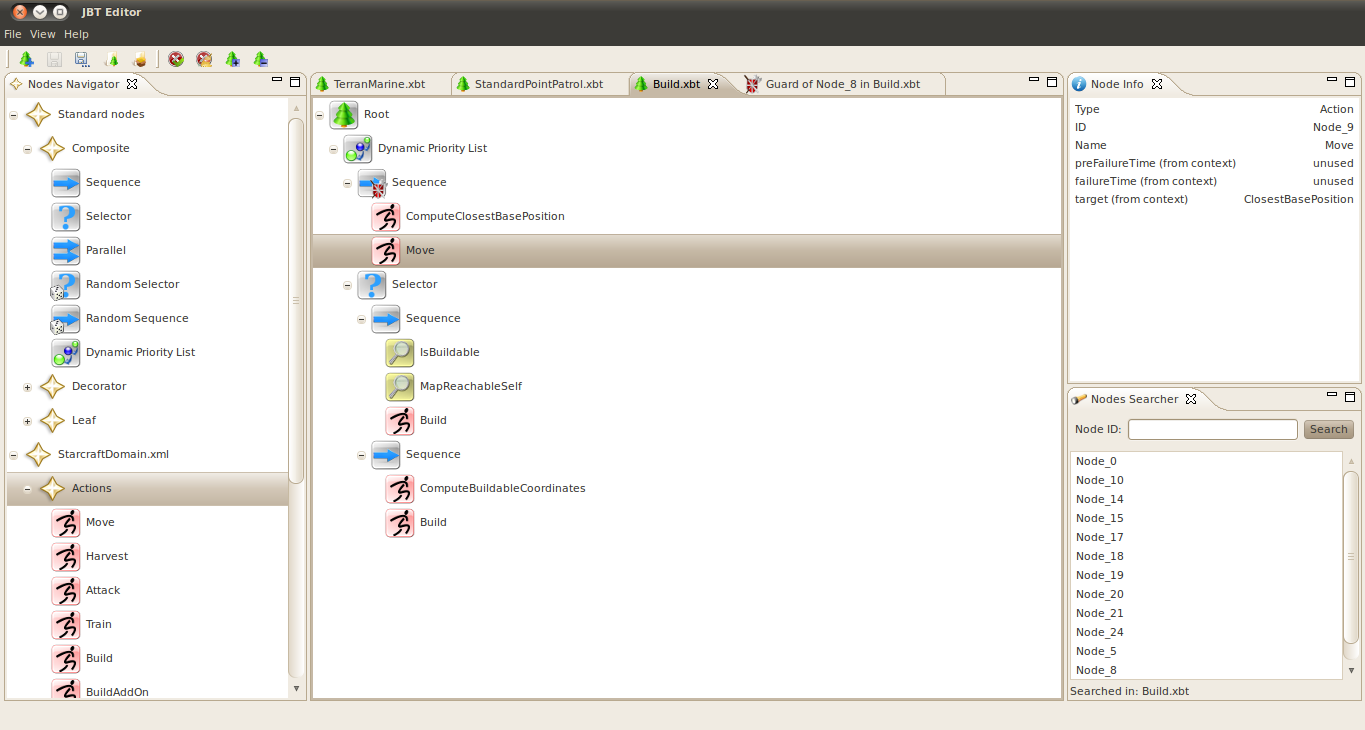
\includegraphics[width=\textwidth]{./Images/JBTEditor.png}
 % JBTEditor.png: 1365x730 pixel, 72dpi, 48.15x25.75 cm, bb=
 \caption{JBT Editor}
 \label{fig:JBTEditor}
\end{figure}

\bibliographystyle{plain}
\bibliography{JBTBib}

\end{document}
